
% Include LaTeX packages
\documentclass[conference]{styles/acmsiggraph}
\usepackage{comment} % enables the use of multi-line comments (\ifx \fi)
\usepackage{fullpage}
\usepackage{enumitem}
\usepackage{amsmath,amsthm,amssymb}
\usepackage{listings}
\usepackage{graphicx}
\usepackage{etoolbox}
\usepackage{verbatim}
\usepackage[dvipsnames]{xcolor}
\usepackage{fancyvrb}
\usepackage{hyperref}
\usepackage{menukeys}
\usepackage{titlesec}
\usepackage{csquotes}
\usepackage{placeins}
\usepackage{algorithm} 
\usepackage{algpseudocode}
\usepackage{unicode-math}
\newcommand{\?}{\stackrel{?}{=}}
\renewcommand\qedsymbol{$\blacksquare$}

% Set additional LaTeX options
\setlength{\parskip}{.8mm}
\setcounter{MaxMatrixCols}{20}
\hypersetup{
	colorlinks=true,
	urlcolor=[rgb]{0.97,0,0.30},
	anchorcolor={0.97,0,0.30},
	linkcolor=black,
	filecolor=[rgb]{0.97,0,0.30},
}

% Define title, author, and affiliation information
\title{\huge PSET 3 \\ \LARGE {CS124: Data Structures and Algorithms \\ Prof. Mitzenmacher}}
\author{\Large Dhilan Ramaprasad \\ dhilanramaprasad@college.harvard.edu}
\pdfauthor{Student Name}

% Redefine \VerbatimInput
\RecustomVerbatimCommand{\VerbatimInput}{VerbatimInput}%
{fontsize=\footnotesize,
 %
 frame=lines, % top and bottom rule only
 framesep=2em, % separation between frame and text
 rulecolor=\color{Gray},
 %
 label=\fbox{\color{Black}\textbf{OUTPUT}},
 labelposition=topline,
 %
 commandchars=\|\(\), % escape character and argument delimiters for commands within the verbatim
 commentchar=* % comment character
}

% Set addditional formatting options
\titlespacing*{\section}{0pt}{5.5ex plus 1ex minus .2ex}{2ex}
\titlespacing*{\subsection}{0pt}{3ex}{2ex}
\setcounter{secnumdepth}{4}
\renewcommand\theparagraph{\thesubsubsection.\arabic{paragraph}}
\newcommand\subsubsubsection{\paragraph}

% Define a convenient norm symbol
\newcommand{\norm}[1]{\left\lVert#1\right\rVert}
\renewcommand{\vec}[1]{\mathbf{#1}}

% Define a macro for hiding answers
\newbool{hideanswers} \setbool{hideanswers}{false}
\newenvironment{answer}{}{}
\ifbool{hideanswers}{\AtBeginEnvironment{answer}{\comment} %
\AtEndEnvironment{answer}{\endcomment}}{}

% Define text formatting for points and normals
\newcommand{\points}[1]{\hfill \normalfont{(\textit{#1pts})}}
\newcommand{\pointsin}[1]{\normalfont{(\textit{#1pts})}}







%%%%%%%%%%%%%%%%%%%%%%%%%%%%%%%%%%%%%%%
%%%%%%%%%%%%%%%%%%%%%%%%%%%%%%%%%%%%%%%
%%%%%%%%%%%%%%%%%%%%%%%%%%%%%%%%%%%%%%%
%%%%%%%%%%%%%%%%%%%%%%%%%%%%%%%%%%%%%%%
%%%%%%%%%%%%%%%%%%%%%%%%%%%%%%%%%%%%%%%

         %  START HERE  %

%%%%%%%%%%%%%%%%%%%%%%%%%%%%%%%%%%%%%%%
%%%%%%%%%%%%%%%%%%%%%%%%%%%%%%%%%%%%%%%
%%%%%%%%%%%%%%%%%%%%%%%%%%%%%%%%%%%%%%%
%%%%%%%%%%%%%%%%%%%%%%%%%%%%%%%%%%%%%%%
%%%%%%%%%%%%%%%%%%%%%%%%%%%%%%%%%%%%%%%

\begin{document}
\maketitle

\textbf{Collaborator}: Benny Paris \\
\textbf{Others:} Esther/Amy

\newpage


%%%%%%%%%%%%%%%%%%
%   Question #1  %
%%%%%%%%%%%%%%%%%%
\section{Risk-Free Currency Exchange}
\subsection{Assumptions:}
\begin{itemize}[label= ---]
    \item We seek to yield a profit by returning to a \textbf{start currency}. If no such return path exists, our relative profit is harder to quantify and could be better expressed by starting from a different currency if there is profit to be made.
    \item By the last item, I assert that in our problem we seek a scenario where if we start at currency $i=1$, we return to it, so our exchange rates will go $r_{i_1,i_2}\cdot r_{i_2,i_3}\cdot...\cdot r_{i_{k-1},i_k}\cdot r_{i_k,i_1}$.
\end{itemize}

\subsection{Goals:}
\begin{enumerate}
    \item Seek out backedges (i.e., find a loop if any exists)
    \item Check to see if any origin paths from a currency node which is the destination of a backedge result in $r_{i,j}\cdot r_{j,i} \textgreater 1$.
    \item The \textbf{Bellman-Ford Algorithm} finds \textit{negative} cycles.  Perhaps transform our \enquote{graph} (wherein nodes represent a currency type and edges represent exchange rates) to a setup where traversal of paths need not require multiplication of exchange rates, $r_{i,j}$, but instead addition (summing) of rates $\implies$ log transform.
    \item Simply return whether a risk-free exchange \textit{exists} (not necessarily finding it).
\end{enumerate}


\subsection{Algorithm:}
Let us set up our currency exchange problem by representing all currencies as nodes on a directed graph.  Exchange rates, if they exist, will populate our graph as directed edges.

\rule{\textwidth}{0.4pt}
\begin{enumerate}
    \item Convert edge-weights to their log equivalents (e.g., substitute $log_2(r_{i,j})$ for $r_{i,j}$).
    \item Negate the entire graph (i.e., change all edge weights to their negative value) and run Bellman-Ford at each vertex to return if there exists a negative cycle (which would reflect a positive cycle in the original graph).  
    \item To be clear, Bellman-Ford needs to be run such that it would indicate a negative cycle, so---given the algorithm---its \enquote{relaxation} process needs to \textbf{iterate $\mathbf{|V|}$ times} \textit{each time} the algorithm is run, rather than $(|V|-1)$ times as assumed in Bellman-Ford when seeking a general shortest path.
\end{enumerate}
\rule{\textwidth}{0.4pt}

\subsection{Proof:}
\subsubsection{The Log Transform:}
First, by direct proof, I show that a log transform is valid.  Consider the following rule of logarithms:
\begin{align}
    log_2(k) < 0, k < 1\\
    log_2(k) = 0, k = 1\\
    log_2(k) > 0, k > 1
\end{align}

Given the problem's original specification:
\begin{align}
    r_{i,j} \cdot r_{j,i} > 1\\
    \therefore log_2(r_{i,j} \cdot r_{j,i}) > 0
\end{align}

So, using the logarithm product rule (which holds for additional inserts of exchange rates, $r$ by converting a logarithmic expression's argument (expressed as a product of values) into a summation of individual logarithmic terms of each value, respectively) we can express our desired path:
\begin{equation} \label{eq:positive_sum}
    log_2(r_{i,j}) + log_2(r_{j,i}) > 0
\end{equation}

Naturally, if we negate our edge weights, we can synonymously multiply the above, equation \ref{eq:positive_sum}, by $-1$ to get:
\begin{equation} \label{eq:neg_log}
    -log_2(r_{i,j}) + -log_2(r_{j,i}) < 0
\end{equation}

Given the validity of the prior steps, we have reduced this problem into a situation where we need to apply the Bellman-Ford algorithm to find a negative cycle (i.e., the sum of edge weights results in some path yields a distance less than 0 as seen in equation \ref{eq:neg_log}).  Bellman-Ford is proven (in course notes) to be a correct method to seek negative cycles. \qedsymbol

\subsection{Run-time Analysis:}
Our initial transformation of edge-weights to their log-2 equivalents takes a constant time per edge $\implies O(|E|)$.  Then, the Bellman-Ford algorithm is applied with run-time $O(|V|\cdot |E|)$ at every vertex.

\rule{\textwidth}{0.4pt}
$$ O(|E|) + O(|V|^2 \cdot |E|)$$
$$ \approx O(|V|^2 \cdot |E|)$$
\rule{\textwidth}{0.4pt}























\newpage

\section{New MST Search}
%%%%%%%%%%%%%%%%%%
%   Question #2  %
%%%%%%%%%%%%%%%%%%
\subsection{Given + Assumptions:}
\begin{itemize}[label= ---]
    \item We are given the original minimum spanning tree, $T$
    \item We are given the whole graph, $G$
\end{itemize}

\subsection{Algorithm:} \\
\rule{\textwidth}{0.4pt}
First, we shall scan simultaneously the original MST and the adjusted tree to find the changed edge.  This can be performed in $O(|E|)$ time.  Next, when the changed edge is identified, remove it from the MST.  Now we have split our graph into sets, let's call them $S$ and $V-S$, seeing as all vertices are contained in the two sets, and we have split the adjusted tree into at least one segment $X$, where $X$ is a subset of some minimum spanning tree, and $S$ has no edge in $X$ crossing between $S$ and $V-S$.  We need to now apply the Cut Property to search for a minimum weight edge crossing between $S$ and $V-S$.  In this scenario, we can take the proof as shown in Lecture 7 to show that we will return a minimum spanning tree of the adjusted graph.\\
\rule{\textwidth}{0.4pt}


\subsection{Satisfy Cut Property Requirements?}
We must show that we satisfy the cut property requirements, namely that our section $X$ is a portion of a minimum spanning tree of the graph.  We can prove by contradiction: suppose that $X$ is not part of the minimum spanning tree of $G$, then there exists a method by which to connect the vertices in $S$ in a better fashion than currently done in $X$ implying that our original MST was not an MST, after all, which contradicts the fact that it was an MST.  So let us now show that we have actually found a way to split and select $S$ and $S-V$ such that no edge crosses.  Suppose the preceding was untrue, thereby an edge crosses $S$ and $S-V$ despite removing an edge from our adjusted tree (specifically, the changed weight edge).  If this is the case, there would be a cycle in the original MST, negating its position as an MST $\implies$ contradiction.  So we can see that we satisfy cut property requirements and can reduce this problem without further proof.

\subsection{Run-time analysis:}
The run-time is composed of two elements:  first the finding of the augmented edge in the MST $O(|E|)$, then the iterations to find the lightest edge between our cut which requires visiting all vertices in one cut and checking edges which connect to the other cut segment $O(|V|)$. \\
\rule{\textwidth}{0.4pt}
$$\implies O(|V| + |E|)$$
\rule{\textwidth}{0.4pt}
























\newpage


\section{Set Cover Family}
%%%%%%%%%%%%%%%%%%
%   Question #3  %
%%%%%%%%%%%%%%%%%%
Take a family of sets such that the number of elements can be represented in the following way:

$$n = k\cdot 2^a$$

where $k=3$ for our initial scenario.

Say there exist an optimal set cover in which $\frac{1}{3}$ of the total elements are covered in subsets $O_1$, $O_2$, $O_3$.  Now take an additional grouping of subsets wherein the first $S_0$ contains $\frac{1}{2}$ of each $O_1$, $O_2$, $O_3$ thereby comprising $\frac{1}{2}$ of the entire set, thus selected first by a greedy algorithm ($S_0$ is of size $k\cdot 2^{a-1}$.  $S_1$ contains $\frac{1}{2}$ of each $O_1$, $O_2$, $O_3$ not already covered by $S_0$ (i.e., $\frac{1}{2}$ of all remaining uncovered elements which is larger than those covered by $O_1$, $O_2$, $O_3$).  This process repeats until there exists 1 element in each $O_1$, $O_2$, $O_3$ which remain uncovered by any set $S_i$ (where $S_i$ is of size $k\cdot 2^{a-i}$, for integer $i \geq 1$).  Thus we must collect the sets $O_1$, $O_2$, $O_3$ which would have been optimal at the start if we collected them first despite their lower coverage percentage of uncovered sets. (See Figure \ref{setcover} for an example where $k=3$.)\\

We collect, then, $a-1+k$ sets which is larger than $log(k\cdot2^a)$ by logarithmic rules:
\begin{align}
    a-1+k > log(k) + a
\end{align}

We have shown that for the example above and fully generalizable, the set cover returned by the greedy algorithm is bounded below by log(n).

\begin{figure}[h!]
    \centering
    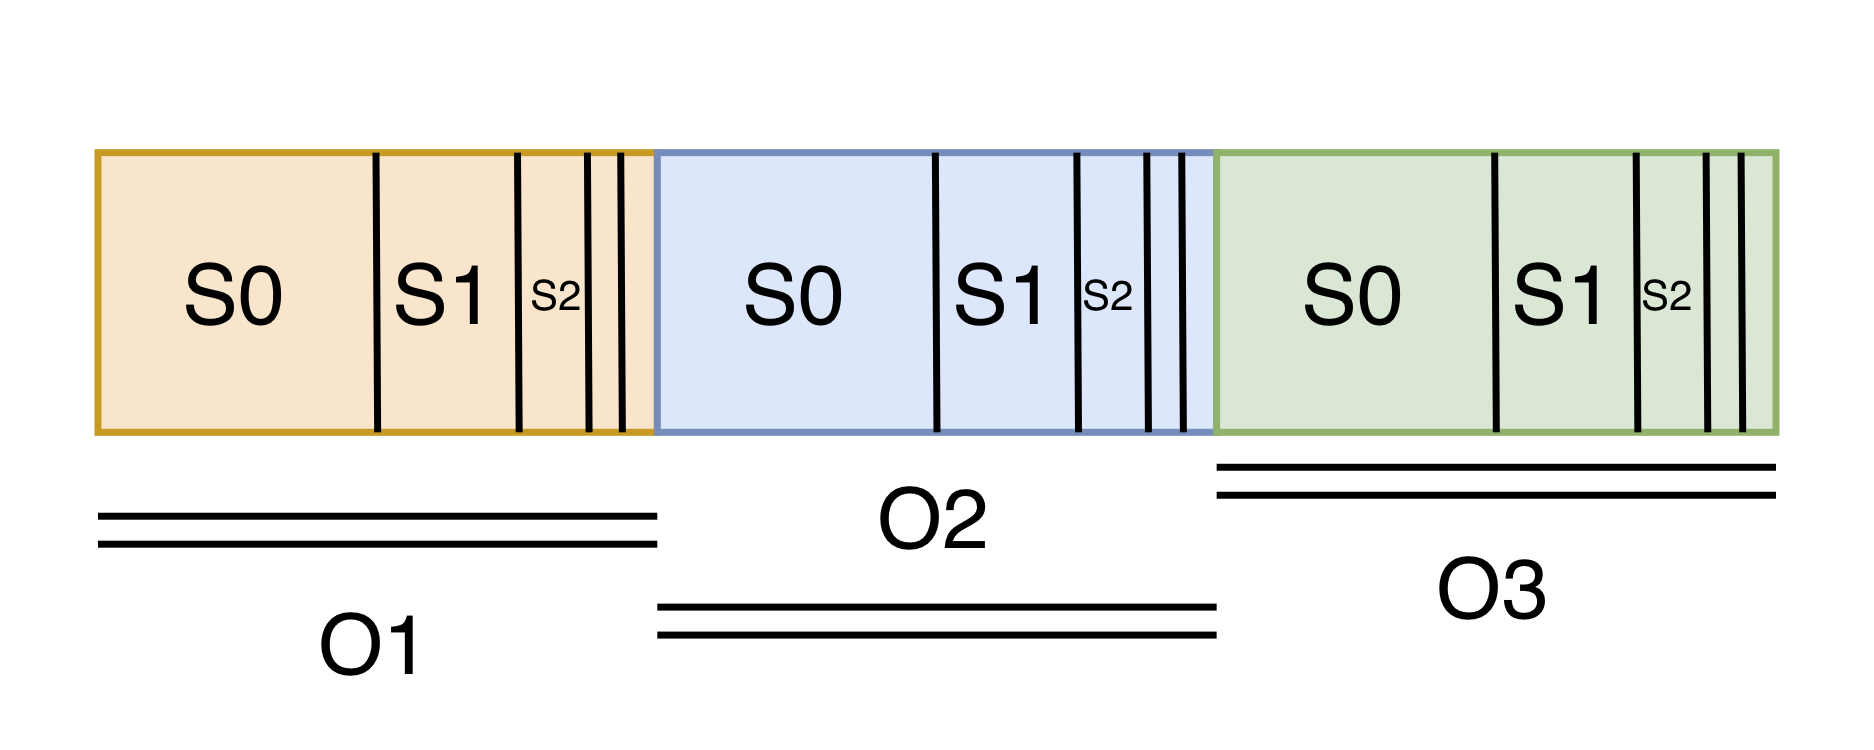
\includegraphics[width=0.6\textwidth]{Problem 5 Figures/p3 fig/CS124 PSET1_3 Diagrams (1).png}
    \caption{$k=3$ Set Cover example}
    Note the divisibility once by three afforded by the $k$ term in $n = k\cdot 2^a$\\ and then the repeated divisibility by 2 after which point given by the power of 2.
    \label{setcover}
\end{figure}
\FloatBarrier





\newpage

\section{Scheduling Jobs}
%%%%%%%%%%%%%%%%%%
%   Question #4  %
%%%%%%%%%%%%%%%%%%
Given a set of jobs $\{j_1, j_2, j_3, ..., j_n\}$ with respective run-times, $r_i$, for sequential processing---but distributable to 2 equivalent machines---we must show that a greedy algorithm of placement of each job successively on the machine with the lower current load yields at worst a $\frac{3}{2}$ performance ratio when compared to the optimal (i.e., minimal run-time) placement of jobs on the two machines.

\subsection{Lower Bounds of Optimal Run-time:} \label{section:lowerBound}
Before continuing further, let's consider the lower bounds of an optimal solution.
\begin{enumerate}
    \item I hold that optimal completion time $\coloneq t_{optimal} \geq r_{max}$ where $r_{max}$ is the largest run-time of a job, $j_i$.  This is clearly true as \textit{some} machine \textbf{must} run the longest job.
    \item Additionally, I assert that $t_{optimal} \geq \frac{1}{2} \sum_{i}r_i$ because the machine with the heavier load \textbf{must} do at least half of the total job load by definition of it being the \enquote{heavier load} machine $\implies$ $t_{optimal} = t_{(completion\ time\ heavy)}$.
\end{enumerate}

\subsection{Upper Bounds of Greedy Run-Time} \label{section:upperBound}
\textbf{First}, I hold that the two machines can, at worst, differ by $r_{max}$ using the greedy allocation algorithm.  Let us show this via induction: 
\begin{enumerate}
    \item In our base case, on the first iteration, no jobs have been placed.  The first job can be at most with of run-time load $r_{max}$ $\implies$ the machine loads can differ at most by $r_{max}$.
    \item Suppose for all iterations $n < (N-1)$ our machine loads differ at most by $r_{max}$ on the $N$th iteration, then, the following scenarios can occur:
    
    \begin{enumerate}
        \item The longest job has already been placed, and---given our greedy algorithm---any next job will go on the machine with lighter load, and seeing as this job, $j_N$ has run-time $r_N < r_{max}$, the load-gap between the machines \textbf{can only narrow}, as the only way the machine with the lighter load can exceed the load of the heavier machine (given their difference at $(N-1)$th iteration is $\leq r_{max}$) would be by adding a load greater than $r_{max}$.
        \item The longest job has not yet been placed (or there exist multiple replicas of this longest job---one of which has not been placed), by our induction hypothesis, the machines' difference at the $(N-1)$th iteration is $\leq r_{max}$, and by our greedy algorithm, we add $r_{max}$ to the machine with the lighter load again which  \textbf{can only narrow} our machines' load gap (irrespective of which machine then takes the lead in heaviness of load) if not nullify the gap entirely
    \end{enumerate}
    $\implies$ for all iterations, using the greedy allocation, our machines differ at most by $r_{max}$.
\end{enumerate}

\textbf{Now}, let's establish some bounds on machine loads at the $(n-1)$th iteration using an average work metric similar to our lower bound of optimal run-time from Section \ref{section:lowerBound}:
\begin{enumerate}
    \item By definition of its being the lighter-loaded machine (must be below average):
    \begin{align} \label{eq:load_light_nminus1}
        load_{light} \leq \frac{\sum_{}^{n-1}{r_i}}{2} \implies load_{light} \leq \frac{r_{total}-r_n}{2}
    \end{align}
    \item By definition of its being the heavier-loaded machine (i.e., above average) and by what was shown above that the machines can differ at most by $r_{max}$: 
    \begin{align} \label{eq:load_heavy_nminus1}
        load_{heavy} \leq \frac{\sum_{}^{n-1}{r_i}}{2} + r_{max} \implies load_{heavy} \leq \frac{r_{total}-r_n}{2} + r_{max}
    \end{align}
\end{enumerate}
Unfortunately, though, this bounding is not tight enough; after all, if we consider the lighter-loaded machine being at its upper bound (i.e., the average of the (n-1) assigned jobs), the heavier machine cannot be $r_{max}$ above this average simply because we have upended the essence of the \enquote{average} now.  To reiterate, the upper bound of the heavier machine, given our loose bounds in Equation \ref{eq:load_heavy_nminus1}, is $r_{max}$ above the average of the (n-1) assigned jobs, and if the machines can only differ by $r_{max}$, the lighter machine \textbf{must} be at the \enquote{average}, but then our \textit{average} no longer remains the so-called average as \textbf{one machine cannot be above average without the other being strictly below average}. \\

Let's make a tighter bound, then wherein we \textit{implicitly} take that the machines can maximally differ by $r_{max}$ but \textbf{explicitly} state tight upper (\enquote{worst-case} bounds):

\begin{enumerate}
    \item The lighter loaded machine:
    \begin{align} \label{eq:load_light_tight}
        load_{light} \leq \frac{\sum_{}^{n-1}{r_i}}{2} - \frac{r_{max}}{2}\implies load_{light} \leq \frac{r_{total}-r_n}{2} - \frac{r_{max}}{2}
    \end{align}
    \item By definition of its being the heavier-loaded machine (i.e., above average) and by what was shown above that the machines can differ at most by $r_{max}$: 
    \begin{align} \label{eq:load_heavy_tight}
        load_{heavy} \leq \frac{\sum_{}^{n-1}{r_i}}{2} + \frac{r_{max}}{2} \implies load_{heavy} \leq \frac{r_{total}-r_n}{2} + \frac{r_{max}}{2}
    \end{align}
\end{enumerate}


Consider, now, the $n$th iteration (i.e., the final job placement).  There exist two cases:
\begin{enumerate}
    \item $r_n = r_{max}$ thereby equation \ref{eq:load_light_tight} transforms (by substitution of $r_n = r_{max}$) to:
    \begin{align}
        load_{(light\ previous\ iteration)} \leq \frac{r_{total}}{2}
    \end{align}
    and equation \ref{eq:load_heavy_tight} can be written similarly:
    \begin{align}
        load_{(heavy\ previous\ iteration)} \leq \frac{r_{total}}{2}
    \end{align}
    such that the machines can, now, be of equal load share at the upper end of this bound---this is an uninteresting case.
    
    \item $r_n < r_{max}$ thereby equation \ref{eq:load_light_tight} transforms to:
    \begin{align}
        load_{(light\ previous\ iteration)} \leq \frac{r_{total}-r_{max}}{2} + \frac{r_{n}}{2}
    \end{align}
    and equation \ref{eq:load_heavy_tight} can be written similarly:
    \begin{align} \label{eq:BIGBOI}
        load_{(heavy\ previous\ iteration)} \leq \frac{r_{total}+r_{max}}{2} - \frac{r_{n}}{2}
    \end{align}
\end{enumerate}

Equation \ref{eq:BIGBOI} is our largest upper bound (i.e., the worst case), then, and it comes in the scenario where the heaviest machine remains the heaviest load (and thereby determines the greedy run-time) after adding the final job. \\

To write this bound without reference $r_n$, we can loosen slightly without any loss of generality (given we're loosening):
\begin{align} \label{eq:LOOSEBOI}
    \mathbf{greedy\ run\ time} \leq \frac{r_{total}+r_{max}}{2}
\end{align}

\newpage
\subsection{Reconciling Worst Case Bounds}
\begin{align} \label{lowerboundOpt}
    t_{optimal} = max\left(\frac{1}{2} \sum_{i}r_i, r_{max}\right)
\end{align}
\begin{align} \label{upperboundGreedy}
    t_{greedy} = \frac{r_{total}+r_{max}}{2}
\end{align}

Let's consider three comprehensive cases, now:
\begin{enumerate}
    \item $r_{max} > \frac{1}{2} \sum_{i}r_i$
    \begin{align} \label{eq:scenario1}
        \frac{ t_{greedy}}{t_{optimal}} = \frac{r_{total}}{2r_{max}} + \frac{1}{2}
    \end{align}
    The expression above is definitively less than 1 ($\implies$ less than $\frac{3}{2}$) because the first term on the right hand side of equation \ref{eq:scenario1} is strictly less than $\frac{1}{2}$ by the supposition $r_{max} > \frac{1}{2} \sum_{i}r_i = \frac{r_{total}}{2}$.
    
    \item $r_{max} < \frac{1}{2} \sum_{i}r_i$
    \begin{align} \label{eq:scenario2}
        \frac{ t_{greedy}}{t_{optimal}} = 1 + \frac{r_{max}}{r_{total}}
    \end{align}
    The expression above is definitively less than $\frac{3}{2}$ because the second term on the right hand side of equation \ref{eq:scenario2} is strictly less than $\frac{1}{2}$ by the supposition $r_{max} < \frac{1}{2} \sum_{i}r_i = \frac{r_{total}}{2}$.
    
    \item $r_{max} = \frac{1}{2} \sum_{i}r_i$
    \begin{align} \label{eq:scenario3}
        \frac{ t_{greedy}}{t_{optimal}} = 1 + \frac{r_{max}}{r_{total}}
    \end{align}
    The expression above is equal to $\frac{3}{2}$ because the second term on the right hand side of equation \ref{eq:scenario3} is $\frac{1}{2}$ by the supposition $r_{max} = \frac{1}{2} \sum_{i}r_i = \frac{r_{total}}{2}$. \\
\end{enumerate}

$\implies$ The greedy strategy yields a completion time at worst still within a factor of $\frac{3}{2}$ of the best possible placement of jobs.$\qed$

\subsection{Example:}
Suppose we have two machines and three jobs where the first two jobs are of length 1 and the third of length 2.  In the best placement, the third job (of length 2) is placed on one machine and the other two jobs (of length 1 each) are placed on the remaining machine $\implies$ run-time of 2.  In the greedy algorithm, if the first two jobs in to be placed are the shorter ones, the machines are loaded each with one of the 1-length jobs, then the 2-length job is placed on a machine $\implies$ run-time of 3; thereby, the factor of $\frac{3}{2}$ is achieved.

\subsection{$m$-machine Generalization}

\subsubsection{Lower Bounds of Optimal, Upper Bounds Greedy:} 
Following our analysis from Sections \ref{section:lowerBound} and \ref{section:upperBound}:
\begin{align} \label{lowerboundOptM}
    t_{optimal} = max\left(\frac{1}{m} \sum_{i}r_i, r_{max}\right)
\end{align}
\begin{align} \label{upperboundGreedyM}
    t_{greedy} = \frac{r_{total}}{m}-\frac{r_{max}}{m} + r_{max}
\end{align}

To clarify, equation \ref{upperboundGreedyM} comes from our earlier analysis of the sole interesting case where $r_n < r_{max}$ (see equation \ref{eq:LOOSEBOI} above). Following the \enquote{three comprehensive cases} analysis performed in equations \ref{eq:scenario1}, \ref{eq:scenario2}, and \ref{eq:scenario3}, I will show (because it shows the strictest bound the interesting case wherein $r_{max} = \frac{1}{m} \sum_{i}r_i = \frac{1}{m} r_{total}$:

\begin{align} \label{eq:scenario1M}
    \frac{t_{greedy}}{t_{optimal}} = 1 + \frac{r_{total}}{m \cdot r_{max}} - \frac{1}{m}\\
    = 2 - \frac{1}{m}
\end{align}


\subsubsection{Family of examples:}
Suppose, with our greedy allocation, we place on every of $m$ machines $(m-1)$ jobs of length 1 and have a single remaining job of length $m$.  The greedy allocation would place the last job such that total run-time is $2m+1$; whereas, a best case placement would spread one of the machine's $(m-1)$ length-1 jobs to each other machine, one per remaining machine, before then placing the long m-length job on a machine by itself $\implies$ run-time is $m$.  The ratio, then, reaches our maximum bound shown above:

$$\frac{t_{greedy}}{t_{optimal}} = \frac{2m-1}{m} = 2 - \frac{1}{m}$$









\newpage


\section{Three-Split $n$-digit Multiplication}
%%%%%%%%%%%%%%%%%%
%   Question #5  %
%%%%%%%%%%%%%%%%%%
\subsection{Assumptions:}
\begin{itemize}[label= ---]
    \item From Piazza @348, \enquote{If n is not divisible by 3, you could imagine left padding the number with 1 or 2 zeros which doesn't change the asymptotics. So for simplicity, feel free to assume that \textbf{n is divisible by 3}.}
    \item From Piazza @369, addition and bit-shift operations can be summarized in a single $O(n)$ term.
\end{itemize}

\subsection{Setup:} \label{section:setup}
Let's split our two $n$-digit numbers (where $n$ is a multiple of 3) into thirds as seen in Figure \ref{fig:thirds}:

\begin{figure}[h]
    \centering
    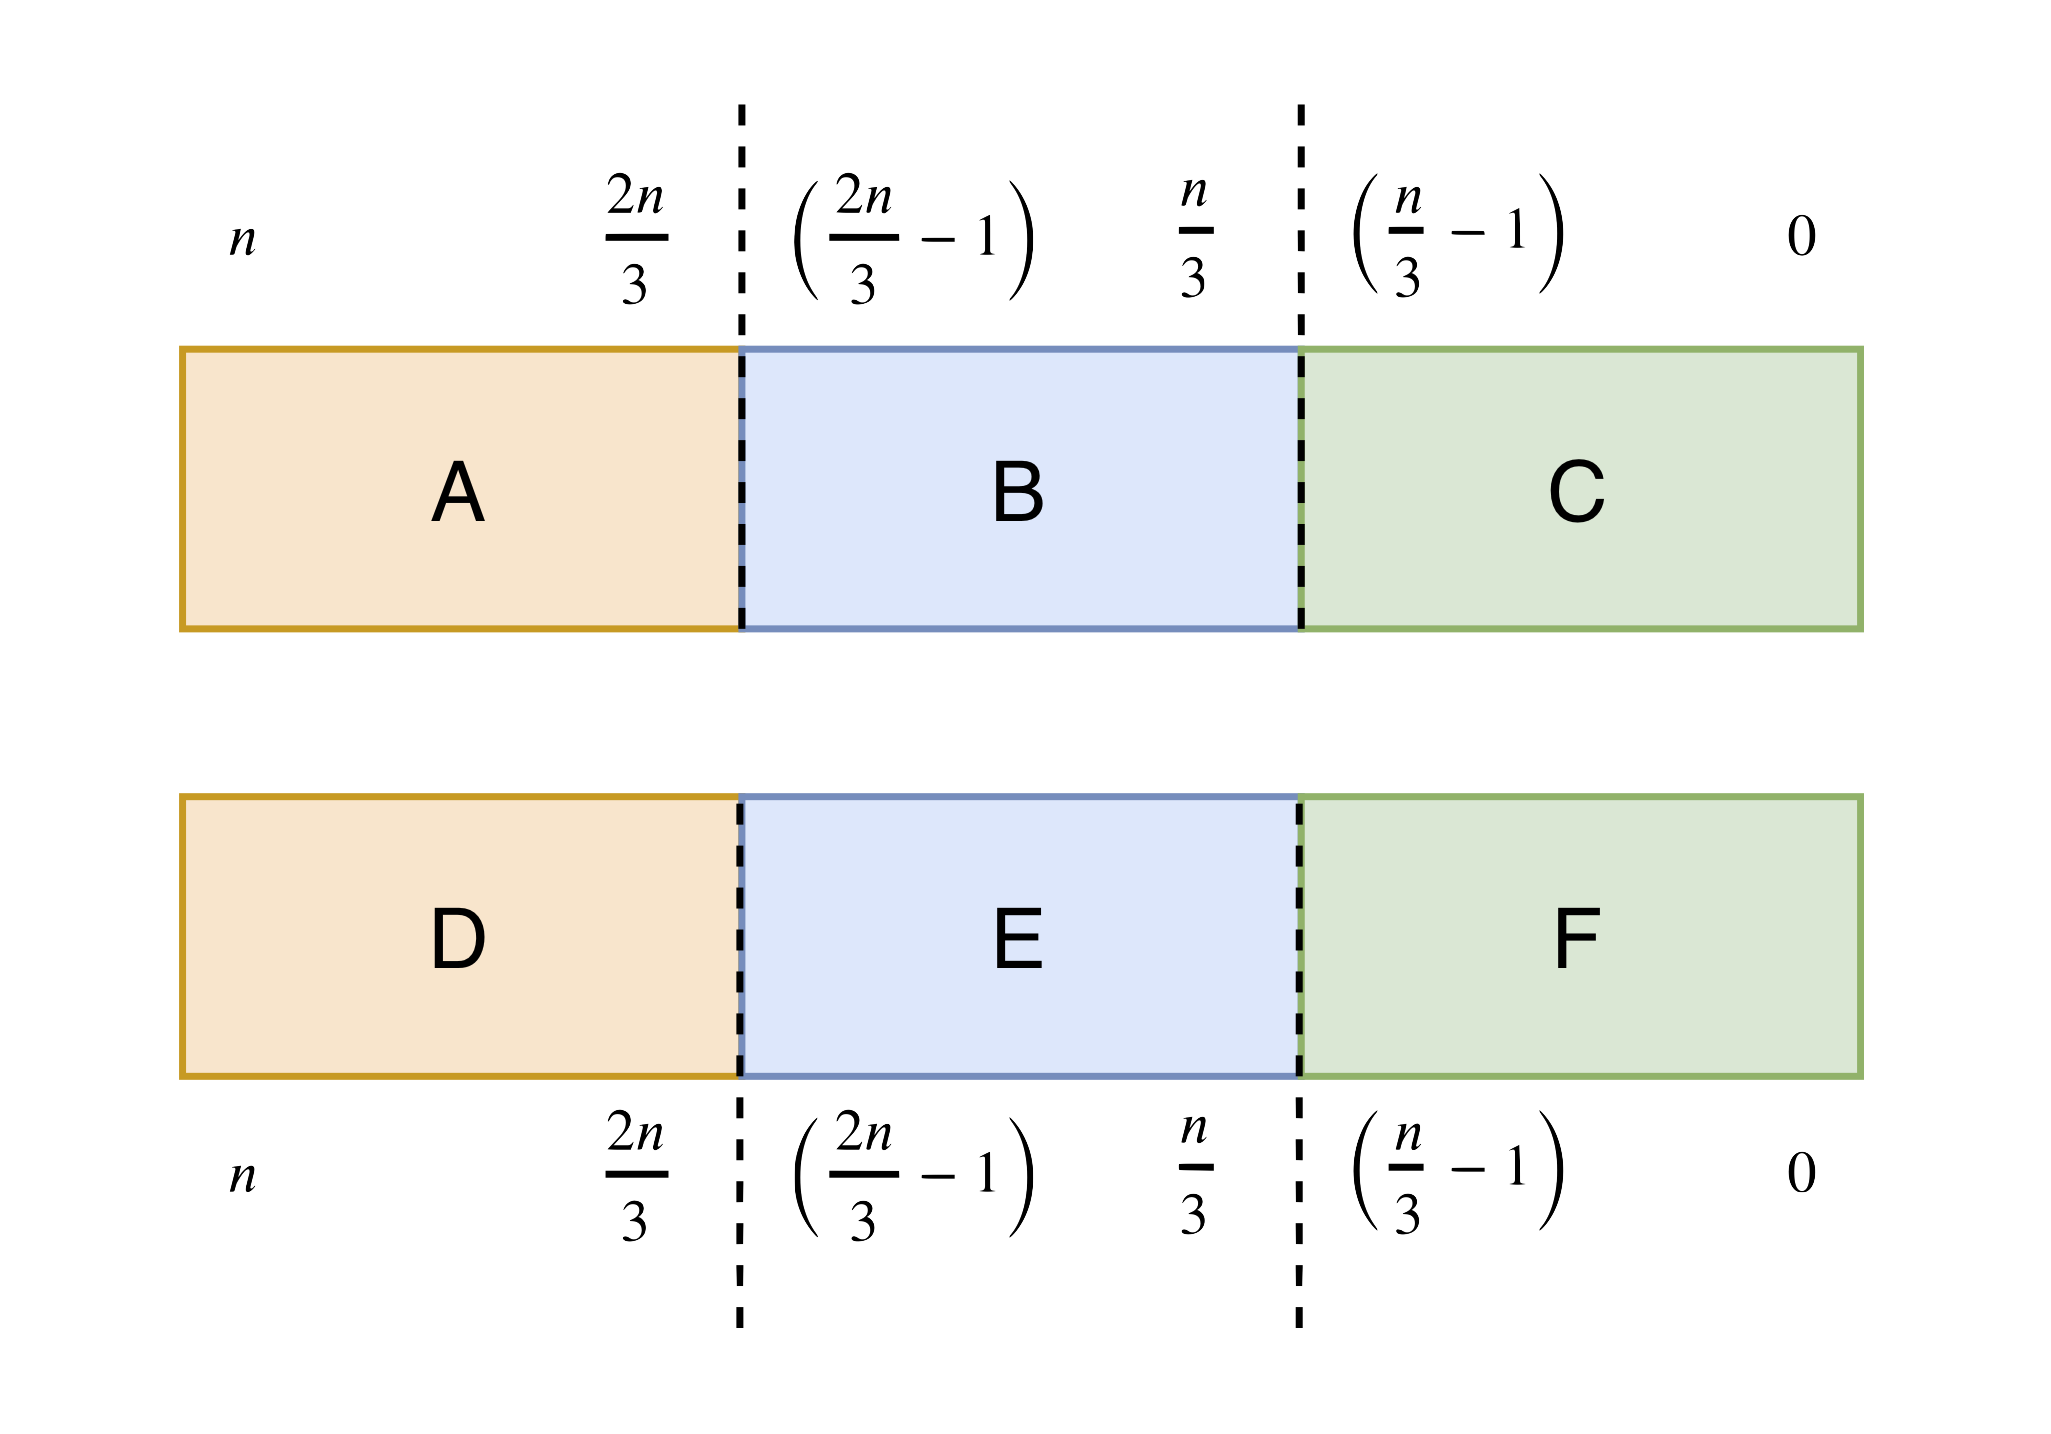
\includegraphics[width=0.6\textwidth]{Problem 5 Figures/CS124 PSET1_3 Diagrams.png}
    \caption{$n$-digit numbers split into thirds}
    \label{fig:thirds}
\end{figure}
\FloatBarrier

Let $x \coloneq \frac{n}{3}$.

\subsection{Multiply!}
We can express our multiplication, now:
\begin{align} \label{eq:unsimplified}
    (a\cdot 10^{2x} + b \cdot 10^{x} + c) \cdot (d\cdot 10^{2x} + e \cdot 10^{x} + f)
\end{align}
Distributing terms of equation \ref{eq:unsimplified}:
\begin{align} \label{eq:distributed}
    (ad\cdot 10^{4x} + ae\cdot 10^{3x} + af\cdot 10^{2x} + bd\cdot 10^{3x} + be\cdot 10^{2x} + bf\cdot 10^{x} + cd\cdot 10^{2x} + ce\cdot 10^{x} + cf)
\end{align}
$\implies$ non-ideal 9 multiplications!  We can resolve by combining like terms of equation \ref{eq:distributed}:
\begin{align} \label{eq:grouping}
    ad\cdot 10^{4x} + (ae+bd)\cdot 10^{3x} + (af+be+cd)\cdot 10^{2x} + (bf+ce)\cdot 10^{x} + cf
\end{align}
Equation \ref{eq:grouping} can be re-written in a manner which minimizes the number of unique products needed:
\begin{align*} \label{eq:we_got_em}
    ad\cdot 10^{4x} + [(a+b)(e+d)-ad-be]\cdot 10^{3x} + [(a+c)(d+f)-ad-cf+be]\cdot 10^{2x} + [(b+c)(e+f)-be-cf]\cdot 10^{x} + cf
\end{align*}

\subsection{Reiterating the Algorithm}
Split the $n$-digit value as in Section \ref{section:setup}.  Then add/multiply as follows: \\
\rule{\textwidth}{0.4pt}
\begin{align*} \label{eq:we_got_em}
    ad\cdot 10^{4x} + [(a+b)(e+d)-ad-be]\cdot 10^{3x} + [(a+c)(d+f)-ad-cf+be]\cdot 10^{2x} + [(b+c)(e+f)-be-cf]\cdot 10^{x} + cf
\end{align*}
\rule{\textwidth}{0.4pt}

Let's now consider the unique multiplications required:
\begin{enumerate}
    \item $a \cdot d$
    \item $b \cdot e$
    \item $c \cdot f$
    \item $(a+b) \cdot (e+d)$
    \item $(b+c) \cdot (e+f)$
    \item $(a+c) \cdot (d+f)$\\
\end{enumerate}
Hooray! It's just 6 multiplies!

\subsection{Run-time Analysis (Part B):}
We can create a recurrence for this multiplication technique as follows:
$$ T(n) = 6T\left(\frac{n}{3}\right) + O(n)$$
Using Master Theorem, we can approximate:
$$O(n^{log_3(6)})$$
Since this is not better than the two-split multiplication $O(n^{log_2(3)})$, I prefer to split into two.

\subsection{Five Multiplications:}
Supposing we could complete the integer multiplication using five unique multiplications, our recurrence could be re-written:
$$ T(n) = 5T\left(\frac{n}{3}\right) + O(n)$$
Using Master Theorem, we can approximate:
$$O(n^{log_3(5)})$$
and since this is better than the two-part split, I would rather split into three if I could reduce to 5 multiplications.

\newpage
\end{document}
